\documentclass[conference]{IEEEtran}
\IEEEoverridecommandlockouts

\usepackage{cite}
\usepackage{amsmath,amssymb}
\usepackage{graphicx}
\usepackage{booktabs}
\usepackage{textcomp}

\begin{document}

\title{Explainable Contextual Emotion Recognition via Text-Guided Chain-of-Thought Reasoning}

% Placeholders: fill in names, affiliation and emails before submission.
\author{\IEEEauthorblockN{N. Q. Sang}
\IEEEauthorblockA{Artificial Intelligence, FPT University\\
sangquang2904@gmail.com}}
\maketitle

\begin{abstract}
Contextual emotion recognition asks which emotions a designated person in an image feels, given the person and the scene. Recent systems let a vision-language model (VLM) reason in text and name the emotions itself, which leaves two problems: the output cannot be scored with mAP against trained classifiers, and the written rationale need not be the reason for the answer. We describe a pipeline that splits these roles. A VLM (Qwen3-VL-4B) only extracts visible person cues, context cues and relations for the target, without naming emotions; a frozen text encoder and a frozen vision encoder feed a small transformer that predicts the 26 EMOTIC categories; modality interventions on the trained model produce an evidence package; and the VLM only verbalizes that package. We check the verbalization automatically for agreement with the measured most important modality, accuracy of cited numbers, emotions named outside the prediction, and ERASER comprehensiveness and sufficiency. On the 7,280 EMOTIC test people, ResNet-50 baselines reach 25.39--27.35 mAP against 17.0 for a constant scorer, and their prediction fits a swapped-in target better in only 40.5\% of 9,988 pairs. Cue extraction for all 34,320 people returns schema-valid JSON for 99.6\%, but 18.9\% of cue sets contain affect words such as ``smiling'' despite the instruction. On the test set the fusion model reaches 28.5 mAP and 32.2 macro-F1 (mean of three seeds); with affect words deleted from the cues it reaches 30.0 and 33.7, above a vision-only variant (27.0, 31.3) and the best ResNet-50 (27.35, 30.9). Affect-free cues beat vision only in paired bootstrap on both a held-out validation half and the test set, while the extra gain of the raw cues on validation does not carry over to test. Over all 1,691 validation and 7,280 test explanations, 99.97\% of cited numbers match the evidence, but the VLM names the person as most important in 99.5\% of cases and agrees with the measured most important modality no more often than always naming the most frequent one; by ERASER its choice is no more faithful than that constant.
\end{abstract}

\begin{IEEEkeywords}
contextual emotion recognition, EMOTIC, vision-language models, multimodal fusion, explanation faithfulness
\end{IEEEkeywords}

\section{Introduction}
Reading how a specific person feels from one image is ambiguous without context. The same posture can fit several emotions, and psychological work argues that expressions alone do not identify emotions reliably~\cite{barrett2019,barrett2011}. The EMOTIC dataset~\cite{kosti2017emotic,kosti2020emotic} cast the task as multi-label recognition of 26 emotion categories for an annotated person in a natural scene. Two-stream CNNs over the person crop and the whole image were the first baselines~\cite{kosti2020emotic}. Later models added context-aware attention~\cite{lee2019caer}, a Frege-principle-based fusion of several contexts~\cite{mittal2020emoticon}, multiple-context awareness~\cite{yang2022heco}, a single-stage decoupled subject--context transformer~\cite{li2024tscnet}, context debiasing~\cite{yang2024debias}, and pre-training on verbal and nonverbal communication~\cite{zhang2023emotionclip}.

Large VLMs changed the recipe. Etesam et al.\ turn images into captions and let an LLM pick labels, and they compare GPT-4V and LLaVA~\cite{etesam2023,etesam2024}. Other studies evaluate or fine-tune VLMs directly~\cite{lei2025lvlm,bhattacharyya2025eve} or feed their descriptions to a trained classifier~\cite{xenos2025vllm}. EmoCoT, a 2026 agentic framework, builds per-person cards and repairs predictions with a verifier~\cite{chen2026emocot}. Text-based reasoning for contextual emotion is therefore not new.

Two problems remain when the VLM itself names the emotions. (i)~A generated label set has no score per label, so authors could not report mAP and compare with CNNs on the metric the CNNs were built for~\cite{etesam2024,lei2025lvlm}. (ii)~A chain-of-thought rationale need not reflect why the answer was produced~\cite{turpin2023,lanham2023,jacovi2020}. Our own pilot (Sec.~\ref{sec:pilot}) adds a third: a structured prompt raised micro-F1 mainly by predicting one frequent label more often.

We therefore keep text in the pipeline but change its role. The VLM is used twice, and neither time does it decide the emotions: first it describes what is visible about the target and the scene, and later it puts into words evidence that was measured on a trained classifier. Recognition is done by a classifier that outputs a probability for every label, so it can be scored like the CNN baselines on the same split.

% PROVISIONAL-CONTRIBUTIONS
Our contributions are:
\begin{enumerate}
\item \textbf{A role-separated pipeline, evaluated once on the test set.} VLM cue extraction without emotion words, frozen BERT and ViT encoders, a transformer that fuses person, context and cue tokens, modality interventions, and VLM verbalization of the resulting evidence (Sec.~\ref{sec:method}). Three-seed comparisons against variants without the cue, context or person token and with affect words deleted from the cues, on a held-out validation half and on the test set, and paired comparisons with ResNet-50 baselines on the same test people (Sec.~\ref{sec:fusion}).
\item \textbf{Automatic checks for grounded explanations, run on every validation-eval and test person.} Modality agreement with a majority-modality control, cited-number accuracy, the rate of emotions named outside the prediction, and ERASER comprehensiveness and sufficiency against the most frequent, a random and the measured modality (Sec.~\ref{sec:explain}, \ref{sec:explresults}).
\item \textbf{A controlled baseline audit on the EMOTIC test set.} ResNet-50 baselines with constant baselines, paired image-level bootstrap, label-policy and label-frequency controls, region masking with a random-box control, and a within-image target swap (Sec.~\ref{sec:baseline}).
\item \textbf{Cue extraction for all 34,320 people.} Parse, schema and truncation rates, cue counts, batched-decoding speed and agreement, and a leakage check for affect words (Sec.~\ref{sec:cues}).
\end{enumerate}
% END-PROVISIONAL
We make no claim that our approach is better than existing systems.

\section{Related Work}
\textbf{Context-aware recognition.} Besides the models listed above, other datasets add whole-body or video context, for example BoLD for bodily expression~\cite{luo2020arbee}. ResNet backbones~\cite{he2016resnet} remain the common starting point for supervised baselines, and we follow that choice for our reference models.

\textbf{VLMs and LLMs for contextual emotion.} Etesam et al.\ first generated captions for the target person and scene and asked an LLM to reason from them in a chain-of-thought style~\cite{etesam2023}. Their follow-up compares captions, GPT-4V, LLaVA and a fine-tuned LLaVA against the EMOTIC CNN~\cite{etesam2024}. In their macro-averaged results LLaVA fine-tuned on the augmented validation set reaches 36.83 F1 against 28.83 for the CNN, and GPT-4V with an engineered prompt reaches 34.47. They state that they could not use mAP and that VLMs struggle to identify the person referred to in a prompt. They also note that captions lack social and object interactions, that there is no ``don't know'' option, and that it is unknown how much of the EMOTIC test set the VLMs saw~\cite{etesam2024}. Yang et al.\ study captions for contextual emotion estimation~\cite{yang2023captions}. Lei et al.\ evaluate zero-shot, few-shot and fine-tuned LVLMs on EMOTIC and HECO; adding chain-of-thought examples raised precision but lowered recall on EMOTIC and reduced performance on HECO~\cite{lei2025lvlm}. Xenos et al.\ feed VLM-generated descriptions to a trained classifier~\cite{xenos2025vllm}, which is the closest design to our first stage. Bhattacharyya and Wang benchmark several VLMs on image emotion~\cite{bhattacharyya2025eve}, and Zhang et al.\ prompt with numbered boxes over all faces~\cite{zhang2024sov}. ELENA narrates embodied emotion with structured outputs~\cite{saim2025elena}. AICA-Bench examines affective image content analysis and an open-vocabulary approach evaluates visual emotion understanding~\cite{she2026aica,wu2025customizing}, and EIBench targets emotion interpretation~\cite{lin2025eibench}. Multimodal LLMs that reason about or explain emotion, mostly in video with audio, include EMER, Emotion-LLaMA, R1-Omni and AffectGPT-RL~\cite{lian2023emer,cheng2024emotionllama,zhao2025r1omni,lian2026affectgptrl}; EmoLLM covers images and videos~\cite{yang2024emollm}. Open-weight VLMs such as Qwen2.5-VL~\cite{bai2025qwen25vl} make it possible to re-run prompts and models.

The closest work is EmoCoT~\cite{chen2026emocot}. We could read only its abstract and reference list on the publisher's page; the full text is behind a paywall. According to the abstract, it uses per-person cards, verifier-guided repair, and evaluates on an EMOTIC-based benchmark and a new multi-person benchmark. Its cards and our cue extraction both describe one person at a time; the difference is that in our pipeline the VLM never outputs the emotion labels.

\textbf{Reasoning and faithfulness.} Chain-of-thought prompting~\cite{wei2022cot} is known to produce explanations that need not reflect the reason for an answer~\cite{turpin2023,lanham2023}. NLP work distinguishes plausibility from faithfulness~\cite{jacovi2020}, calls for rigorous evaluation of interpretability~\cite{doshivelez2017}, and measures faithfulness with tests such as simulatability~\cite{hase2020las,chen2023cs}, counterfactual or intervention tests~\cite{atanasova2023,lanham2023}, and self-consistency checks for vision-language decoders~\cite{parcalabescu2024}. For images, counterfactual edits of cited objects have been proposed~\cite{ding2026edct,menzat2026vct}. In emotion research, ERV checks agreement between explanation and label~\cite{rha2026erv}; FACR intervenes on facial action units~\cite{huynh2026facr}; OPPO masks modalities and probes claims~\cite{han2026oppo}; DSPO masks the image region its reasoning cites and down-weights interpretations that the image does not support~\cite{ye2026dspo}; AffectOmni audits grounding after the fact~\cite{wang2026affectomni}. These works test whether a model's own rationale is faithful. We avoid part of that problem by measuring the evidence on the classifier first and asking the VLM only to report it; what remains to test is whether the report stays within the evidence.

\textbf{Labels, scoring and target grounding.} Mart{\'\i}nez-Miwa and Castel{\'a}n re-annotated a 1,120-image EMOTIC subset with eight emotion groups and filtered each image's votes with a Z-score threshold, which changed label counts and agreement~\cite{martinez2023reliability}. For scoring, token-probability readouts have been used for multi-label text emotion~\cite{ma2025mlc}, and reading the answer from the logits has been reported to beat generated answers on a facial emotion benchmark~\cite{hallmen2026readout}; our classifier gives per-label probabilities directly instead. For target grounding, consistency under person swaps has been proposed for visual commonsense reasoning~\cite{kim2023vcr}; we apply a swap test to our emotion baselines.

\section{Methodology}\label{sec:method}
Each sample is one annotated person $i$ in an image $I$ with bounding box $b_i$ and a multi-hot target $y_i\in\{0,1\}^{26}$. The pipeline has five stages.

\textbf{1) Cue extraction.} The target is marked with a red box on $I$, and Qwen3-VL-4B-Instruct\footnote{Hugging Face model \texttt{Qwen/Qwen3-VL-4B-Instruct}.} is asked to return one JSON object with at most three short visible person cues (face, pose, gesture, clothing, action), at most three context cues (scene, objects, other people), at most two relations involving the target (e.g.\ ``target facing person\_2''), and one sentence describing what is visibly happening. The prompt forbids naming or inferring any emotion and never lists the 26 categories, so the label set cannot leak through the prompt. Decoding is greedy with at most 192 new tokens, and images are resized to at most 409,600 pixels. To make the full set feasible, prompts are decoded in batches with left padding; the batch size is chosen on people that already have cues, as the fastest size whose schema rate stays at or above 95\%. Outputs that do not match the schema are replaced by a single fallback node.

\textbf{2) Encoding.} Each cue, relation and the situation sentence become a node with one of four types; a sample has at most nine nodes. A frozen BERT-base encoder\footnote{\texttt{google-bert/bert-base-uncased}, first-token embedding, 32 tokens.} maps each node text to a 768-d vector. A frozen ViT-B/16 pre-trained on ImageNet\footnote{\texttt{torchvision} \texttt{vit\_b\_16}, \texttt{IMAGENET1K\_V1} weights.} maps the person crop and the whole image to 768-d vectors $v^p_i$ and $v^c_i$. All features are computed once and cached.

\textbf{3) Fusion.} Node vectors are projected to $d=256$, a type embedding is added, and a two-layer transformer encoder (8 heads) followed by masked mean pooling gives one cue vector $g_i$. Because every node attends to every other node, this is a fully connected cue graph without labelled edges; we do not claim structured relational reasoning. A second two-layer transformer takes four tokens, a learned class token, $W_pv^p_i$, $W_cv^c_i$ and $g_i$, each with a modality embedding, and a linear head on the class token outputs logits $z_i\in\mathbb{R}^{26}$ and probabilities $\hat p_i=\sigma(z_i)$. Training uses binary cross-entropy with per-label positive weights $\min(10,\max(1,N^-_k/N^+_k))$, AdamW (learning rate $3\times10^{-4}$, weight decay $10^{-4}$), batch size 32 and 20 epochs.

\textbf{4) Evidence.} For each modality $m\in\{\text{person},\text{context},\text{cue}\}$ the corresponding token is set to zero in the trained model, giving $\hat p_i^{(-m)}$. The drop $\Delta_{ik}^{m}=\hat p_{ik}-\hat p_{ik}^{(-m)}$ for each predicted label $k$ is stored with the cues in an evidence package. Zeroing a token is an intervention at the level of modalities only and moves the input off the training distribution; it does not attribute the decision to pixels or to individual cues.

\textbf{5) Verbalization.} The VLM receives the evidence package and must return \texttt{\{"most\_important\_modality", "explanation"\}}, explaining the prediction using only the supplied evidence and citing probability changes. The VLM still sees the image in this step, so it could add reasons from the image; the checks below are designed to detect that.

\subsection{Evaluation protocol}\label{sec:explain}
\textbf{Splits.} Training uses all 23,706 PAMI training people. The 3,334 validation people are split by image into a dev half (1,643 people; checkpoint, per-label threshold and $k$ selection) and an eval half (1,691 people; reporting), each with 1,044 images, so people from one image never fall into both halves. The 7,280 test people (4,389 images) are scored only with models, thresholds and $k$ fixed on dev. The first test run covered the full, no-cue and affect-free variants; the no-context and no-person variants, the ResNet comparison and the test explanations were added afterwards without changing any setting, and the rerun reproduced the earlier test numbers exactly.

\textbf{Recognition.} We report mAP, macro-F1 and micro-F1 with per-label thresholds chosen on dev, a constant top-$k$ baseline whose $k$ and label order are chosen on dev, and paired image-level bootstrap intervals of macro-F1 differences (2,000 draws). To test what each input contributes, the same fusion model is retrained without the cue token (vision only), without the context token, without the person token, and with 22 affect words deleted from every cue before encoding. Each variant is trained with seeds 42--44 and reported as mean and standard deviation; bootstrap intervals compare the seed-42 runs. The seed-42 run of the full model is the main checkpoint, which produces the evidence packages.

\textbf{Explanations.} For an explanation $e$ of sample $i$, let $m^\star_i=\arg\max_m \frac{1}{|K_i|}\sum_{k\in K_i}\Delta^m_{ik}$ be the modality with the largest mean drop over predicted labels $K_i$. We report: (a)~\emph{modality agreement}, the share of explanations whose stated modality equals $m^\star_i$, next to the share obtained by always naming the most frequent $m^\star$; (b)~\emph{cited-number accuracy}, the share of decimal numbers or percentages in $e$ that match a probability, a probability without a modality, or a drop in the package within 0.006; and (c)~the share of explanations that name one of the 26 emotions outside $K_i$. (d)~We also report the two faithfulness metrics of ERASER~\cite{deyoung2020eraser}, with the stated modality $\hat m_i$ as the rationale: comprehensiveness $\frac{1}{|K_i|}\sum_{k\in K_i}(\hat p_{ik}-\hat p_{ik}^{(-\hat m_i)})$, the drop when the rationale is removed (higher is more faithful), and sufficiency $\frac{1}{|K_i|}\sum_{k\in K_i}(\hat p_{ik}-\hat p_{ik}^{(\hat m_i\text{ only})})$, the drop when only the rationale is kept (lower is more faithful). Both are compared with always naming the most frequent $m^\star$, with a random modality, and with $m^\star_i$ itself. These checks are cheap and automatic; they test consistency with the evidence, not whether the classifier's reasons are correct.

\section{Experiments and Results}
All numbers come from our own runs on the extended EMOTIC release with union labels unless stated otherwise.

\subsection{EMOTIC label statistics}\label{sec:data}
We use the extended release with 34,320 annotated people. Table~\ref{tab:labels} gives the number of labels per person under two policies. The \emph{union} keeps every label chosen by any annotator; this equals the official combined categories for all validation and test people. The \emph{majority} policy keeps labels with more than half of the annotators' votes. Training people have one annotator, so the two policies coincide there. In validation, 52.4\% of union labels were chosen by one annotator only, and in test 69.7\%.

\begin{table}[t]
\caption{EMOTIC label statistics (our recount of the official annotations).}
\label{tab:labels}
\centering
\footnotesize
\begin{tabular}{lrrrrr}
\toprule
Split & People & Annot./ & \multicolumn{2}{c}{Labels/person} & 1-vote \\
 & & person & union & majority & share \\
\midrule
Train & 23,706 & 1.00 & 1.96 & 1.96 & -- \\
Val & 3,334 & 4.81 & 6.16 & 1.48 & 52.4\% \\
Test & 7,280 & 2.69 & 4.42 & 1.37 & 69.7\% \\
\bottomrule
\end{tabular}
\end{table}

A model trained on about two labels per person (Table~\ref{tab:labels}, Sec.~\ref{sec:data}) is evaluated against four to six. The label policy therefore affects every comparison below. Multi-person images add a second issue: in test, 996 of 4,994 same-image pairs (19.9\%) have non-empty majority label sets with no label in common, so a model that ignores which person is meant cannot match both people.

\subsection{Reference baselines on the test set}\label{sec:baseline}
We trained ResNet-50 baselines in the style of Kosti et al.~\cite{kosti2020emotic}: person crop only, whole image only, and both encoders concatenated, each with a 512-unit MLP head, binary cross-entropy, AdamW (learning rate $10^{-4}$), 30 epochs, 224-pixel inputs and seed 42 (Fig.~\ref{fig:pilot}a shows validation mAP per epoch). The checkpoint with the best validation mAP was kept, per-label thresholds and the constant baseline were chosen on validation, and the test set was evaluated once.

\begin{figure*}[!t]
\centering
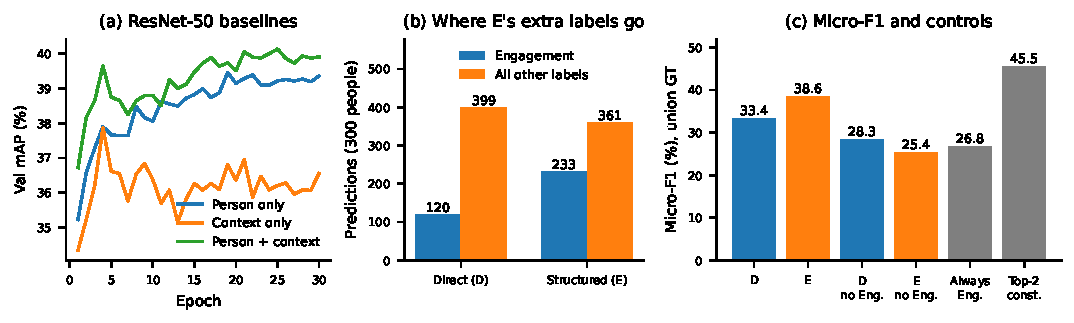
\includegraphics[width=\textwidth]{figures/fig_pilot.pdf}
\caption{(a)~Validation mAP per epoch of the three ResNet-50 baselines. (b)~Number of predicted labels in the VLM pilot (300 people): Engagement versus all other labels, for the direct (D) and structured (E) prompts. (c)~Pilot micro-F1 against union labels, for D and E, for D and E with Engagement removed, for always predicting Engagement, and for a constant top-2 label baseline.}
\label{fig:pilot}
\end{figure*}

\begin{table}[t]
\caption{ResNet-50 baselines on the EMOTIC test set (7,280 people, union labels). Thresholds and $k$ chosen on validation. Pred./p.: predicted labels per person (true: 4.42).}
\label{tab:baseline}
\centering
\footnotesize
\setlength{\tabcolsep}{4pt}
\begin{tabular}{lcccc}
\toprule
Model & mAP & Macro-F1 & Micro-F1 & Pred./p. \\
\midrule
Person only & 25.39 & 23.07 & 44.60 & 2.85 \\
Context only & 27.35 & 30.94 & 53.11 & 7.52 \\
Person + context & 25.97 & 20.79 & 42.87 & 2.29 \\
Constant (top-26) & 16.98$^\dagger$ & 25.12 & 29.03 & 26.00 \\
\bottomrule
\end{tabular}

\vspace{2pt}
{\scriptsize $^\dagger$mAP of any constant scorer equals the mean label prevalence.}
\end{table}

Table~\ref{tab:baseline} shows that all three models are well above a constant scorer in mAP but only context-only beats the constant baseline in macro-F1. The F1 ranking mostly reflects how many labels each model predicts: context-only predicts 7.52 labels per person and wins on recall, while person + context predicts 2.29 and has the highest micro-precision (62.8\%). Paired bootstrap confirms that the macro-F1 gaps are not noise: context-only minus person + context is $+$10.1 points (95\% CI 9.1 to 11.2) and person-only minus person + context is $+$2.3 (1.5 to 3.1). In mAP, which does not depend on thresholds, the spread is only 2 points. Without the frequent label Engagement, mAP falls to 23.1, 25.0 and 23.6, and person + context drops from 28.3 mAP on single-person images to 23.8 on images with three or more people. With majority labels, mAP is 12.6, 15.0 and 12.8.

\textbf{Region masking.} On the person + context model we zeroed (i)~the person crop and the target box in the whole image, (ii)~everything outside the target box, and (iii)~the person crop and a random box of the target's size. Test mAP fell by 5.62, 1.26 and 5.02 points respectively. The random-box control shows that almost all of the person effect comes from losing the person crop; hiding the target's own region in the whole image adds only 0.60 points over hiding a random region. Removing the whole context costs 1.26 points.

\textbf{Target swap.} For 9,988 ordered pairs of people in 1,783 multi-person test images we kept the whole image and replaced the person crop with that of the other person. The prediction matched the new target's labels better than the old target's in 40.5\% of pairs, tied in 23.0\%, and matched the old target better in the remaining 36.6\%; mean sample-F1 was 0.387 with the new target and 0.373 with the old one. The baseline therefore barely tracks which person it is asked about, which motivates the target-specific cues in our pipeline.

\subsection{Pilot: letting the VLM name emotions}\label{sec:pilot}
Before designing the pipeline we ran Qwen2.5-VL-3B-Instruct~\cite{bai2025qwen25vl} on 300 validation people from 279 images (seed 42, greedy decoding, Tesla T4). The target was marked with a red box. In the \emph{direct} prompt (D) the model chose from the 26 labels; in the \emph{structured} prompt (E) it first listed person cues, context cues and the situation, then the emotions. Intervals come from a paired bootstrap over images.

\begin{table}[t]
\caption{VLM pilot, union labels (300 validation people). Intervals: paired image-level bootstrap, 95\%. True labels per person: 6.16.}
\label{tab:pilot}
\centering
\footnotesize
\setlength{\tabcolsep}{4pt}
\begin{tabular}{lccc}
\toprule
 & D & E & E$-$D [95\% CI] \\
\midrule
Macro-F1 & 15.8 & 17.1 & $+$1.2 [$-$0.6, $+$3.0] \\
Micro-F1 & 33.4 & 38.6 & $+$5.2 [$+$3.2, $+$7.0] \\
Predicted labels / person & 1.73 & 1.98 & -- \\
Parse rate (\%) & 100 & 98.67 & -- \\
Seconds / sample & 1.0 & 4.76 & -- \\
\bottomrule
\end{tabular}
\end{table}

E has higher micro-F1, but its macro-F1 gain is not distinguishable from zero (Table~\ref{tab:pilot}). Engagement is the most frequent label (288 of 300 people); D predicts it for 120 people and E for 233 (Fig.~\ref{fig:pilot}b). Without Engagement, micro-F1 is 28.3 for D and 25.4 for E, a difference of $-$2.9 points (CI $-$4.8 to $-$1.0), and a constant top-2 baseline reaches micro-F1 45.5 against 38.6 for E (Fig.~\ref{fig:pilot}c). The pilot is small (one 3B model, one seed), but it showed that the structured rationale did not make the VLM a better labeller, and that generated label sets are hard to compare without per-label scores. This is why the VLM in our pipeline describes and reports but does not label.

\subsection{Cue extraction}\label{sec:cues}
Cue extraction with the prompt of Sec.~\ref{sec:method} was run for all 23,706 training, 3,334 validation and 7,280 test people. The first 2,275 training people in annotation order were decoded one at a time on a Tesla T4 (6.29 seconds per person over the first 1,420); the others were decoded in batches of 48 on an NVIDIA A100 and an NVIDIA H100. In the benchmark of the reported run on the H100, 48 people per batch took 0.22 seconds per person, against 0.27 for 32 and 0.84 for 16, with peak memory of 16.2~GB. Batched decoding is not equivalent to single-sample decoding: for the first 48 training people, the parsed batched output equalled the stored single-sample output for 28, while all 48 still matched the schema; over four runs of this benchmark the count varied from 24 to 28. Table~\ref{tab:cues} summarizes the training and validation outputs; for the test people, decoded in batches of 48 on the H100, 99.99\% of outputs parse, 99.63\% match the schema and none is truncated. The schema failures we inspected had both cue lists empty although the situation sentence was filled. Relations are the weakest part: almost a quarter of the outputs have none.

\begin{table}[t]
\caption{Qwen3-VL-4B cue extraction on all 27,040 training and validation people.}
\label{tab:cues}
\centering
\footnotesize
\begin{tabular}{lr}
\toprule
Measure & Value \\
\midrule
Parsed as JSON & 100.0\% \\
Matches schema & 99.65\% \\
Truncated at the token limit & 0.0\% \\
Person / context cues per sample & 3.00 / 2.99 \\
Relations per sample (none) & 0.86 (23.4\%) \\
Cue sets with an affect word & 18.4\% \\
Seconds per person, T4, single (first 1,420) & 6.29 \\
Seconds per person, H100, batch 48 & 0.22 \\
\bottomrule
\end{tabular}
\end{table}

The prompt forbids emotion words, yet 18.4\% of valid cue sets contain at least one word from a list of 22 affect terms. Most are ``smiling'' (6,099 occurrences), which is arguably a visible facial cue, but ``engaged'' appears 507 times and is nearly the label Engagement, and ``focused'' 143 times. Such words can carry label information from the VLM into the classifier. As a control we delete these 22 words from every cue and re-encode the cues; this changes 18.9\% of the 34,320 cue sets, and the resulting variant is compared in Sec.~\ref{sec:fusion}.

\subsection{Fusion model, variants and test results}\label{sec:fusion}
With BERT and ViT features cached, one training run takes 20 epochs of about 6 seconds on the H100. Table~\ref{tab:fusion} gives every variant on the eval half (1,691 people, 6.18 union labels per person) and on the test set (7,280 people, 4.42), together with the constant baseline and the ResNet-50 baselines of Sec.~\ref{sec:baseline}; Fig.~\ref{fig:fusion} shows the training curves and test mAP.

\begin{table*}[t]
\caption{Fusion model variants on the validation eval half and on the test set (union labels), mean $\pm$ standard deviation over seeds 42--44. Checkpoint, thresholds and $k$ chosen on the dev half. Pred./p.: predicted labels per person on test (true: 4.42). The ResNet-50 rows repeat Table~\ref{tab:baseline}; their thresholds were chosen on the whole validation split.}
\label{tab:fusion}
\centering
\footnotesize
\begin{tabular}{lccccccc}
\toprule
 & \multicolumn{3}{c}{Eval half (1,691 people)} & \multicolumn{4}{c}{Test (7,280 people)} \\
\cmidrule(lr){2-4}\cmidrule(lr){5-8}
Variant & mAP & Macro-F1 & Micro-F1 & mAP & Macro-F1 & Micro-F1 & Pred./p. \\
\midrule
Full (person, context, cue) & 40.5$\pm$0.5 & 42.6$\pm$1.1 & 64.3$\pm$1.6 & 28.5$\pm$1.2 & 32.2$\pm$1.0 & 51.3$\pm$1.8 & 8.69 \\
No cue token (vision only) & 37.5$\pm$0.4 & 40.4$\pm$0.2 & 61.3$\pm$0.7 & 27.0$\pm$0.1 & 31.3$\pm$0.2 & 48.4$\pm$0.7 & 10.29 \\
No context token & 40.1$\pm$0.6 & 43.2$\pm$0.5 & 62.7$\pm$0.6 & 29.8$\pm$0.4 & 33.4$\pm$0.1 & 50.1$\pm$0.7 & 9.68 \\
No person token & 39.8$\pm$0.6 & 43.1$\pm$0.6 & 62.7$\pm$0.6 & 30.4$\pm$0.3 & 33.9$\pm$0.4 & 50.0$\pm$0.8 & 9.86 \\
Cues without affect words & 39.7$\pm$0.1 & 43.5$\pm$0.3 & 62.1$\pm$0.7 & 30.0$\pm$0.2 & 33.7$\pm$0.1 & 49.3$\pm$0.7 & 10.23 \\
Constant (top-26) & 23.8$^\dagger$ & 32.6 & 38.4 & 17.0$^\dagger$ & 25.1 & 29.0 & 26.00 \\
\midrule
ResNet-50, person only & -- & -- & -- & 25.39 & 23.07 & 44.60 & 2.85 \\
ResNet-50, context only & -- & -- & -- & 27.35 & 30.94 & 53.11 & 7.52 \\
ResNet-50, person + context & -- & -- & -- & 25.97 & 20.79 & 42.87 & 2.29 \\
\bottomrule
\end{tabular}

\vspace{2pt}
{\scriptsize $^\dagger$Mean label prevalence of the split.}
\end{table*}

\begin{figure*}[!t]
\centering
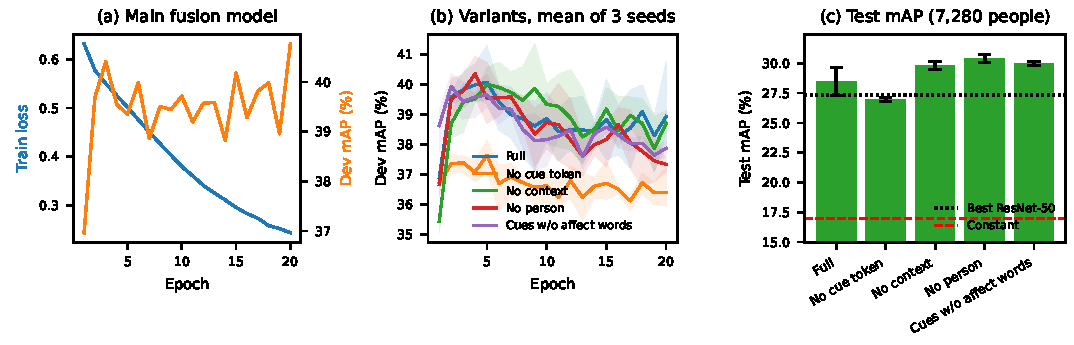
\includegraphics[width=\textwidth]{figures/fig_fusion.pdf}
\caption{(a)~Train loss and dev mAP per epoch of the main fusion model (seed 42). (b)~Dev mAP per epoch of the five variants, mean of three seeds with the min--max range shaded. (c)~Test mAP of the variants (mean and standard deviation over three seeds) against the best ResNet-50 (context only) and the constant scorer.}
\label{fig:fusion}
\end{figure*}

\textbf{Eval half.} Removing the cue token costs 2.9 mAP and 2.2 macro-F1 points on average, several times the seed spread of the vision-only runs, and the vision-only dev curve stays below all others in every epoch (Fig.~\ref{fig:fusion}b). Removing the context or the person token costs at most 0.7 mAP and raises macro-F1 slightly, so once the target-specific cues are present either visual token adds little. Deleting affect words from the cues costs 0.7 mAP but not macro-F1 (43.5 against 42.6), and the affect-free model beats vision only by 2.8 macro-F1 points on the seed-42 runs (95\% CI 0.7 to 5.2).

\textbf{Test set.} Every variant is well above the constant scorer (full minus constant on seed 42: $+$5.8 macro-F1, CI 4.8 to 6.7), but the eval ranking does not carry over. The full model has the largest seed spread, and its seed-42 run, the main checkpoint, is its weakest on test (26.8 mAP against 29.4 and 29.2). On seed means the full model is 1.5 mAP above vision only, and the no-context, no-person and affect-free variants are 1.3 to 2.0 mAP above the full model, differences of the order of the full model's own spread. On the seed-42 runs, full minus vision only is $-$0.3 macro-F1 (CI $-$1.1 to $+$0.5), and full minus no context, no person and affect-free cues is $-$2.3, $-$3.2 and $-$3.0, all with intervals that exclude zero; the weak seed-42 full run contributes to these three gaps. The comparison that holds on both splits and for every seed is affect-free cues against vision only: $+$3.0 test mAP and $+$2.4 test macro-F1 on seed means, and $+$2.7 macro-F1 on the seed-42 runs (CI 1.9 to 3.4), against $+$2.8 on the eval half. Visible cues without affect words therefore add information beyond the frozen image features on unseen people, whereas the further eval gain of the raw cues did not generalize.

All variants predict 8.7 to 10.3 labels per test person against 4.42 true ones, because thresholds were set on dev, which has 6.13 labels per person; the main checkpoint has 43.8\% micro-precision and 69.7\% micro-recall on test. F1 therefore depends on label count, and mAP is the more reliable comparison. The main checkpoint reaches 40.5 mAP, 41.3 macro-F1 and 66.5 micro-F1 on the eval half and 26.8, 30.9 and 53.8 on test. Its per-label test AP ranges from 85.4 for Engagement and 76.4 for Happiness to 5.1 for Fear and 2.4 for Embarrassment.

\textbf{Training noise.} Mean dev mAP of every variant peaks between epochs 2 and 5 and is 1.1 to 3.0 points lower at epoch 20, while the training loss keeps falling (Fig.~\ref{fig:fusion}a,b). The main run instead stays between 38.8 and 40.4 dev mAP from epoch 2 to 19 and peaks at epoch 20 (40.8), so checkpoint selection depends on dev noise of about two points. An earlier pass of the full, no-cue, no-context and no-person variants with the same seeds but a different data-loader random state gave eval mAP 40.9, 38.1, 39.8 and 40.7; the two passes differ by up to 0.9 mAP, so differences below one point should not be read as effects.

\textbf{Against ResNet-50.} On the same test people every pipeline variant has a higher mean mAP (27.0 to 30.4) than all three ResNet-50 baselines (25.39 to 27.35), and the vision-only variant, which uses frozen ImageNet ViT features, is level with the fine-tuned context-only ResNet. In macro-F1 on seed 42, the full model is level with context-only ResNet ($-$0.1, CI $-$1.1 to $+$1.0) and above person only ($+$7.8, CI 6.7 to 8.7) and person + context ($+$10.1, CI 9.1 to 11.0); the affect-free model is above all three, by $+$2.9 (CI 2.0 to 3.9) against context only. With majority labels, test mAP is 13.2 for the main checkpoint and 15.4 for the affect-free seed-42 model, against 12.6 to 15.0 for the ResNets. This comparison is not fully controlled: ResNet thresholds were chosen on the whole validation split with one seed, the ResNets fine-tune their backbone while our encoders are frozen, and the VLM that writes the cues was pre-trained on data we cannot inspect.

\subsection{Explanation checks}\label{sec:explresults}
Qwen3-VL-4B verbalized the evidence package of the main checkpoint for every eval and test person, with greedy decoding, at most 256 new tokens and batches of 32 (the first 30 eval people one at a time). Table~\ref{tab:expl} gives the checks; an explanation is usable when it parses and names one of the three modalities.

\begin{table}[t]
\caption{Explanation checks for the main checkpoint on every eval and test person. ERASER scores are mean probability drops over predicted labels: comprehensiveness ($\uparrow$) removes the named modality, sufficiency ($\downarrow$) keeps only that modality.}
\label{tab:expl}
\centering
\footnotesize
\setlength{\tabcolsep}{3pt}
\begin{tabular}{lrr}
\toprule
 & Eval & Test \\
\midrule
Explanations generated / usable & 1,691 / 1,667 & 7,280 / 7,193 \\
Truncated at the token limit & 1.42\% & 1.09\% \\
Stated modality: person / context / cue & 1,660 / 7 / 0 & 7,158 / 35 / 0 \\
Measured top: person / context / cue & 633 / 672 / 362 & 2,793 / 2,735 / 1,665 \\
Modality agreement & 38.3\% & 38.8\% \\
\quad always the most frequent modality & 40.3\% & 38.8\% \\
Cited numbers & 8,188 & 35,560 \\
\quad found in the evidence & 99.99\% & 99.97\% \\
Names an emotion outside the prediction & 1.74\% & 1.99\% \\
\midrule
Comprehensiveness: stated modality & 0.072 & 0.077 \\
\quad most frequent / random modality & 0.078 / 0.066 & 0.077 / 0.070 \\
\quad measured top modality & 0.157 & 0.159 \\
Sufficiency: stated modality & 0.123 & 0.125 \\
\quad most frequent / random modality & 0.120 / 0.133 & 0.125 / 0.134 \\
\quad measured top modality & 0.045 & 0.047 \\
\bottomrule
\end{tabular}
\end{table}

The VLM copies the evidence faithfully: on the eval half 99.99\% of the 8,188 cited numbers match a probability or a drop in the package within 0.006, and 1.74\% of explanations name an emotion outside the prediction. It does not report which modality the measurements single out. It names the person in 99.6\% of usable eval explanations although the person is the measured top modality for only 38.0\% of people, and its modality agreement (38.3\%) is below that of always naming the most frequent modality (40.3\%). ERASER gives the same picture: the comprehensiveness (0.072) and sufficiency (0.123) of the stated modality lie between those of a random modality and of the most frequent one, far from the 0.157 and 0.045 of the measured top modality. On the test set the measured top modality is most often the person (2,793 of 7,193 usable explanations, against 2,735 for context and 1,665 for cue), and the VLM again names the person in 99.5\%, so its agreement (38.8\%), comprehensiveness (0.077) and sufficiency (0.125) are practically those of always naming the person (38.8\%, 0.077, 0.125). Paired image bootstrap gives stated minus most-frequent modality agreement of $-$2.0 points on eval (95\% CI $-$7.0 to $+$3.1) and $-$0.04 on test ($-$0.18 to $+$0.10), and comprehensiveness of $-$0.006 on eval ($-$0.016 to $+$0.003) and 0.0000 on test ($-$0.0002 to $+$0.0003); against a random modality, comprehensiveness is higher by 0.006 on eval (0.001 to 0.011) and 0.007 on test (0.005 to 0.010). The stated modality is thus slightly better than a random one only because it is nearly always the person, and no better than a constant choice. Cited numbers stay grounded on test as well (99.97\% of 35,560), and 1.99\% of test explanations name an emotion outside the prediction.

\section{Discussion and Limitations}
\textbf{What the cues add.} The ResNet baselines barely change their prediction when the person crop is swapped, so target-specific text was a plausible place to help. On the eval half the cue token gives the largest single gain, but on the test set the raw cues add little over vision only, while the same cues with 22 affect words deleted add 2.2 mAP on eval and 3.0 on test. One reading is that words such as ``engaged'' and ``smiling'' let the classifier lean on the VLM's own affect judgment, which fits the validation annotations better than the test annotations, whose labels are sparser (4.42 against 6.16 per person) and more often chosen by a single annotator (69.7\% against 52.4\% of union labels). We have not tested this reading. Either way, the evidence that visible cues help rests on the affect-free variant. Dropping the context or person token does not hurt on eval and helps on test, so with cues present the three-token model may have more capacity than the data supports; we kept the full model as the main checkpoint because that choice was fixed before the test run.

\textbf{What the explanations show.} Separating decision and verbalization makes the number and emotion checks pass almost everywhere: the VLM does not invent numbers or emotions outside the prediction. The modality check fails on both splits: the VLM nearly always calls the person most important, whatever the measured drops say, and by ERASER its choice is no more faithful than a constant one. Either the VLM cannot aggregate several probability drops into one argmax, or it prefers the modality it finds most plausible from the image, which is the unfaithful behaviour the design was meant to avoid. The check could be passed by computing $m^\star_i$ in code and giving it to the VLM, but then the VLM would only rephrase, so we report the failure as it is.

\textbf{Comparisons.} F1 on EMOTIC is dominated by how many labels a model predicts: our variants predict about twice as many labels per test person as the annotations contain, because thresholds were set on dev with denser labels. We therefore rely on mAP and on paired bootstrap over the same people. The pipeline is above the ResNet baselines in test mAP, but the two sides differ in threshold split, seeds, backbone training and pre-training data, so this shows that the design is competitive with a standard supervised baseline, not that it is better than published systems.

\textbf{Limits of the design.} The cue encoder is a fully connected set of nodes, not a scene graph. Zeroing a modality token is a coarse intervention with distribution shift. The checks in Sec.~\ref{sec:explain} test consistency with the evidence and would not detect evidence that is itself misleading. Cues for 2,275 training people come from single-sample decoding and the rest from batched decoding, whose output equalled the single-sample output for only 50--58\% of the people we compared. Three seeds per variant are few: the full model's test mAP ranges from 26.8 to 29.4 across seeds, and two passes with the same seeds differ by up to 0.9 eval mAP. The ResNet baselines use one seed each. Rerunning the whole notebook from the cached cues reproduced every number exactly.

\section{Conclusion}
We described a pipeline in which a VLM extracts visible cues and verbalizes measured evidence while a trained classifier makes the decision, together with automatic checks, including ERASER comprehensiveness and sufficiency, for whether the verbal explanation stays within the evidence. A test-set audit of ResNet-50 baselines showed that F1 rankings follow the number of predicted labels, that masking the person is barely worse than masking a random region, and that predictions hardly follow a swapped target. A pilot of direct VLM labelling showed gains driven by one frequent label. On the 7,280 test people the pipeline reaches 26.8 to 30.9 mAP across variants and seeds, above the ResNet-50 baselines. Cues help reliably only after affect words are deleted from them, and that variant gives 30.0 test mAP and 33.7 macro-F1. On every eval and test person the verbalized explanations cite numbers from the evidence but name the person as most important almost regardless of the measurements, so their modality claims are no more faithful than a constant. A modality claim computed from the evidence instead of by the VLM, a cue prompt that blocks affect words at generation time, and more seeds are the next steps.

\bibliographystyle{IEEEtran}
\bibliography{refs}

\end{document}
